% Outcome results. Every number comes from results/analysis.json (sha 61a293a2...), written by analyze.py after the
% single unseal (results/unsealed.json, sha 149c8a73...), or from tables generated from it by tables_results.py.

\subsection{Regime checks before the finals}\label{sec:regimechecks}
\paragraph{Language-model overfitting gate}
The protocol required the language-model regime to overfit. The final validation NLL of the tuned reference model had
to end at least 0.02 nats/token above its minimum over the ten evaluations. On the first corpus (1.0M tokens, about eight
epochs) validation NLL was still falling at the last evaluation, so the gap was 0. After the single prespecified
fallback (corpus halved to 0.5M tokens, about 16 epochs over the same 977 steps), the gap was 0.008. The regime is therefore data-limited and
multi-epoch, but it overfits only mildly, and the protocol proceeds without a further fallback. The language-model
learning rate selected for the reference arm, $5\times10^{-4}$, is used by every arm.

\paragraph{Selection}
The prespecified level-selection rules chose AD@0.20, DK@0.05, RA@0.05, HU@0.05, Mixout 0.9 and label smoothing 0.2
in the encoder. They chose AD@0.20, DK@0.20, RA@0.05, HU@0.05 and residual dropout 0.2 in the LM. The strongest
tuned control was label smoothing (LS@0.2) in the encoder and DropKey (DK@0.20) in the LM. CapDrop was not tuned and
ran only at its prespecified operating point, $\ell=0.10$. This is conservative against the method: in the LM, both
tuned controls that beat it were selected at $\ell=0.20$. No top-4 deletion arm can reach that level there
(Section~\ref{sec:census}).

\subsection{Confirmatory and secondary tests}\label{sec:confirmatory}
Table~\ref{tab:confirmatory} and Figure~\ref{fig:forest} report the two families.

% Generated by tables_results.py from results/analysis.json; do not edit by hand.
\begin{table}[t]
\centering
\caption{Confirmatory family F1 (Holm over six tests) and secondary family F2. Differences are first arm minus second
arm; lower is better, so a negative difference favours the first arm. Encoder (E): test Brier, 95\% two-level bootstrap CI, co-criterion =
temperature-scaled Brier difference. LM (L): final-step test NLL (nats/token), 95\% CI by inverting the sign-flip
test, co-criterion = test NLL at the best-validation step. $p$: exact two-sided sign-flip test over ten folds or seeds
(minimum 0.002). Student contrasts S-a and S-b use test Brier.}
\label{tab:confirmatory}
\footnotesize
\setlength{\tabcolsep}{3pt}
\resizebox{\linewidth}{!}{\begin{tabular}{llcccccl}
\toprule
ID & Contrast & Diff. & 95\% CI & Co-crit. & $p$ & $p_{\mathrm{Holm}}$ & Verdict\\
\midrule
H1-E & HB@0.10 $-$ HF@0.10 & $-$0.005 & [$-$0.031, +0.009] & $-$0.003 & 0.432 & 0.863 & Inconclusive\\
H2-E & HB@0.10 $-$ RA@0.05 & $-$0.006 & [$-$0.030, +0.015] & $-$0.005 & 0.457 & 0.863 & Inconclusive\\
H3-E & HB@0.10 $-$ LS@0.2 & +0.132 & [+0.106, +0.159] & +0.009 & 0.002 & 0.012 & calibration only\\
\addlinespace
H1-L & HB@0.10 $-$ HF@0.10 & $-$0.045 & [$-$0.047, $-$0.042] & $-$0.034 & 0.002 & 0.012 & Better\\
H2-L & HB@0.10 $-$ RA@0.05 & $-$0.032 & [$-$0.035, $-$0.029] & $-$0.025 & 0.002 & 0.012 & Better\\
H3-L & HB@0.10 $-$ DK@0.20 & +0.058 & [+0.054, +0.063] & +0.056 & 0.002 & 0.012 & Worse\\
\midrule
\multicolumn{8}{l}{\emph{Secondary family F2 (separate Holm correction)}}\\
S-HBvsHU-E & HB@0.10 $-$ HU@0.10 (E) & $-$0.027 & [$-$0.054, $-$0.002] & $-$0.016 & 0.016 & 0.094 & Inconclusive\\
S-RBvsRA-E & RB@0.10 $-$ RA@0.10 (E) & $-$0.001 & [$-$0.022, +0.021] & +0.001 & 0.959 & 1.000 & Inconclusive\\
S-HBvsHU-L & HB@0.10 $-$ HU@0.10 (L) & $-$0.022 & [$-$0.025, $-$0.020] & $-$0.021 & 0.002 & 0.018 & Better\\
S-RBvsRA-L & RB@0.10 $-$ RA@0.10 (L) & +0.066 & [+0.053, +0.081] & +0.070 & 0.002 & 0.018 & Worse\\
S-a & S-HB@0.10 $-$ S-HU@0.10 & +0.016 & [$-$0.003, +0.036] & +0.011 & 0.006 & 0.041 & Inconclusive\\
S-b & S-HB@0.10 $-$ S-N & +0.000 & [$-$0.012, +0.013] & +0.001 & 0.926 & 1.000 & Equivalent\\
S-interaction-E & (HB$-$HF)$-$(RB$-$RA) (E) & $-$0.009 & -- & -- & 0.359 & 1.000 & Inconclusive\\
S-EUG & evidence-use gap, HB $-$ N & $-$0.012 & -- & -- & 0.363 & 1.000 & Inconclusive\\
S-flip & flip rate, HB $-$ N & +0.011 & -- & -- & 0.078 & 0.391 & Inconclusive\\
\bottomrule
\end{tabular}}
\end{table}


\begin{figure}[t]
\centering
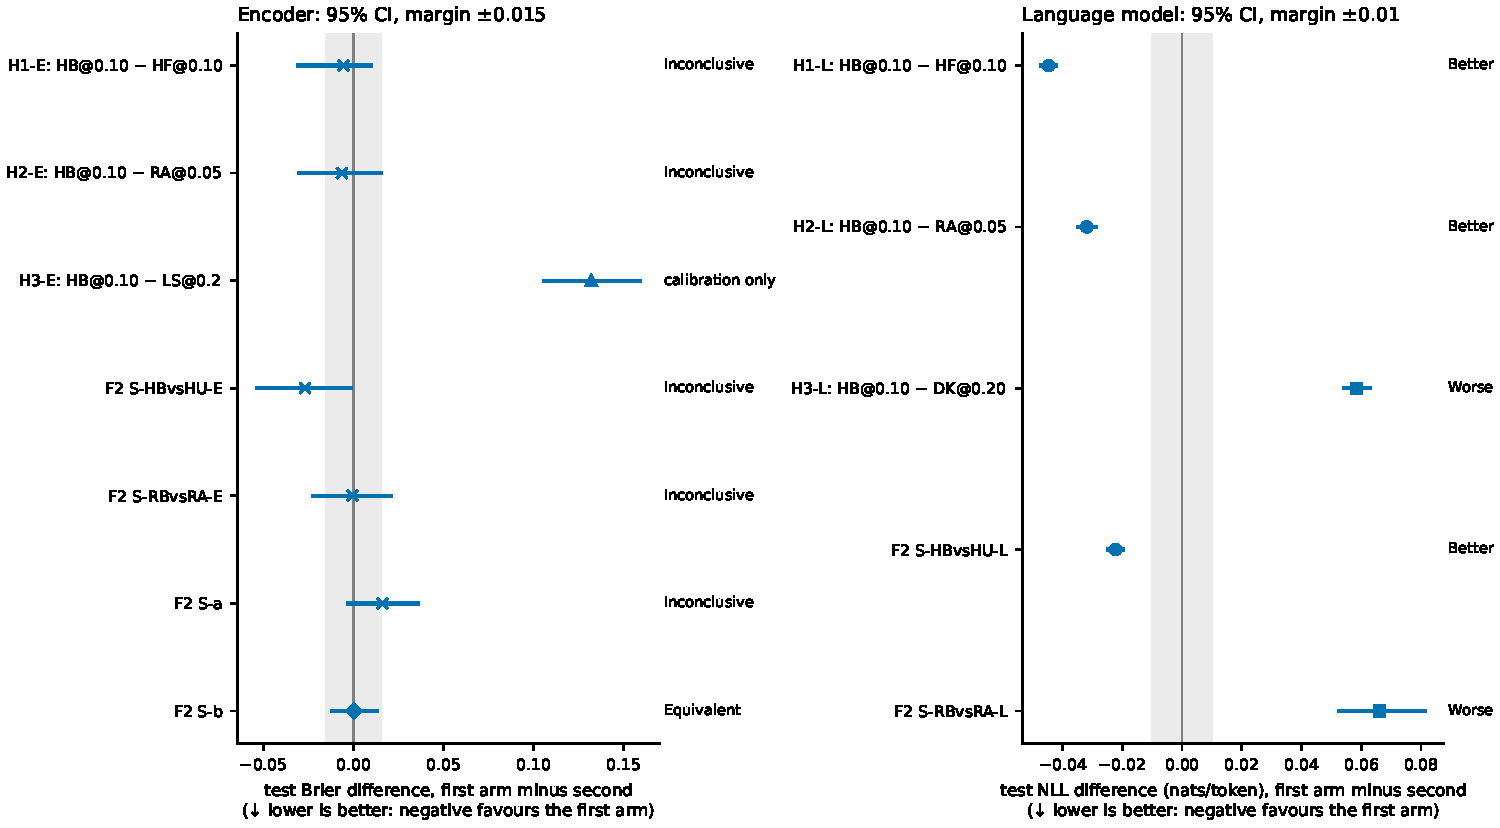
\includegraphics[width=\linewidth]{figures/fig_forest.pdf}
\caption{Confirmatory (H1--H3) and secondary (F2) contrasts with 95\% intervals and the equivalence margins (grey).
Left: encoder, test Brier. Right: language model, final-step test NLL. Verdicts follow the preregistered rules;
``calibration only'' means that raw Brier differs after Holm correction but temperature-scaled Brier does not.}
\label{fig:forest}
\end{figure}

\paragraph{Encoder (PubMedQA)}
None of the three encoder contrasts supports a claim that CapDrop is better. Against fixed-$\alpha$ deletion (H1-E), the mean
difference in test Brier was $-0.005$, with a 95\% interval of $[-0.031, 0.009]$ and Holm-adjusted $p=0.86$. Against
the tuned Relaxed Attention (H2-E), it was $-0.006$, with interval $[-0.030, 0.015]$ and Holm $p=0.86$. Both are
inconclusive. Neither a difference nor equivalence within $\pm0.015$ Brier can be claimed, because the
between-fold standard deviations of the paired differences (0.021 and 0.026) are larger than the margin allows at ten units.
Against label smoothing (H3-E), CapDrop's raw Brier was higher by 0.132 (Holm $p=0.012$). After temperature
scaling, however, the difference shrank to 0.009 and was no longer significant (raw $p=0.072$). The verdict is therefore
``calibration only''. Label smoothing produces better-calibrated probabilities (ECE 0.115 versus 0.301), and a
single temperature fitted on 50 development questions removes almost all of that advantage. Accuracy differed by
0.7 points.

\paragraph{Language model}
All three LM contrasts were decisive, and every one of the ten seeds had the same sign. CapDrop lowered final-step
test NLL relative to fixed-$\alpha$ deletion (H1-L) by 0.045 nats/token, with 95\% interval $[-0.047, -0.042]$ and Holm $p=0.012$.
The best-validation-step difference was 0.034, so the verdict is Better. This is the opposite of the registered
expectation. Because $\delta=0.83\ge0.5$, the census-based rule had registered ``HB not better'' for the LM
(Section~\ref{sec:census}). The test was two-sided, so the verdict stands, but the prediction behind it failed in the
LM. CapDrop also beat the tuned Relaxed Attention (H2-L) by 0.032 nats/token (Better). It was worse than the
strongest tuned control, DropKey at $\ell=0.20$ (H3-L), by 0.058 nats/token (Worse).

\paragraph{Secondary family}
In the LM, CapDrop beat unbudgeted top-4 deletion at the same mean displacement (S-HBvsHU-L) by 0.022 nats/token
(Holm $p=0.018$, Better). Under common random numbers, the two arms delete from the same candidate keys. In the encoder,
the same contrast favoured CapDrop by 0.027 Brier (raw $p=0.016$), but it did not survive the Holm correction
($p=0.094$, Inconclusive). TV-budgeted relaxation was worse than fixed-coefficient relaxation in the LM, by 0.066
nats/token (S-RBvsRA-L, Worse), and indistinguishable from it in the encoder. The $2\times2$ interaction in the
encoder, the evidence-use gap and the flip rate showed no effect (Holm $p\ge0.39$). In the distilled six-layer
students, the contrast S-HB$-$S-HU favoured the unbudgeted arm by 0.016 Brier. Its Holm $p$ was 0.041, but the
two-level interval included zero ($[-0.003, 0.036]$), so the verdict is Inconclusive. S-HB and the student without
attention regularization were equivalent within $\pm0.015$ Brier (S-b).

\subsection{All arms}\label{sec:allarms}
Tables~\ref{tab:arms_encoder} and \ref{tab:arms_lm} report every final arm, and Figure~\ref{fig:dose} places
them against realized displacement.

% Generated by tables_results.py from results/analysis.json; do not edit by hand.
\begin{table}[t]
\centering
\caption{PubMedQA test results by arm (BiomedBERT, ten folds; mean, with the between-fold SD of Brier in parentheses).
TS-Brier: Brier after temperature scaling fitted on each run's development fold. EUG: evidence-use gap (full minus
question-only accuracy, points). Flip: flip rate under a label-differing mismatched abstract (\%). $\bar D$: realized mean
displacement at the end of training. $\downarrow$: lower is better; $\uparrow$: higher is better. Q0 is trained on questions only and is scored here with the abstract; on its own
input format its accuracy is reported in the text. The majority-class accuracy is 55.2\%.}
\label{tab:arms_encoder}
\footnotesize
\setlength{\tabcolsep}{3pt}
\resizebox{\linewidth}{!}{\begin{tabular}{lccccccccc}
\toprule
Arm & Brier$\downarrow$ & TS-Brier$\downarrow$ & Acc.\ (\%)$\uparrow$ & Macro-F1$\uparrow$ & AUROC$\uparrow$ & ECE$\downarrow$ & EUG & Flip & $\bar D$\\
\midrule
N & 0.620 (0.022) & 0.483 & 67.0 & 0.503 & 0.718 & 0.303 & 16.0 & 58.2 & --\\
AD@0.20 & 0.638 (0.028) & 0.497 & 65.6 & 0.507 & 0.713 & 0.306 & 13.0 & 61.4 & 0.200\\
DK@0.05 & 0.632 (0.021) & 0.490 & 66.1 & 0.507 & 0.721 & 0.308 & 13.8 & 59.1 & 0.050\\
RA@0.05 & 0.626 (0.037) & 0.489 & 66.5 & 0.508 & 0.719 & 0.300 & 14.0 & 59.6 & 0.050\\
RA@0.10 & 0.635 (0.038) & 0.492 & 66.0 & 0.509 & 0.714 & 0.307 & 14.3 & 60.6 & 0.099\\
RB@0.10 & 0.634 (0.038) & 0.492 & 65.7 & 0.513 & 0.715 & 0.306 & 13.5 & 61.5 & 0.100\\
HU@0.05 & 0.629 (0.027) & 0.490 & 66.5 & 0.515 & 0.717 & 0.303 & 14.8 & 60.3 & 0.052\\
HU@0.10 & 0.647 (0.030) & 0.500 & 64.9 & 0.509 & 0.717 & 0.311 & 11.6 & 62.6 & 0.102\\
HF@0.10 & 0.630 (0.025) & 0.491 & 66.2 & 0.514 & 0.717 & 0.303 & 13.4 & 61.2 & 0.105\\
HB@0.10 & 0.620 (0.031) & 0.484 & 66.9 & 0.509 & 0.717 & 0.301 & 14.9 & 59.3 & 0.099\\
DB@0.10 & 0.630 (0.030) & 0.490 & 66.1 & 0.502 & 0.719 & 0.307 & 14.9 & 59.1 & 0.100\\
LS@0.2 & 0.488 (0.016) & 0.475 & 67.6 & 0.490 & 0.713 & 0.115 & 15.5 & 56.3 & --\\
MX@0.9 & 0.541 (0.022) & 0.485 & 66.3 & 0.472 & 0.717 & 0.201 & 15.6 & 54.9 & --\\
RDROP@0.5 & 0.632 (0.027) & 0.493 & 66.2 & 0.512 & 0.715 & 0.309 & 14.1 & 59.8 & 0.100\\
Q0 & 1.032 (0.272) & 0.725 & 30.4 & 0.228 & 0.528 & 0.447 & $-$18.9 & 36.8 & --\\
L0 & 0.574 (0.004) & 0.572 & 55.1 & 0.240 & 0.501 & 0.043 & 10.9 & 12.7 & 0.100\\
\bottomrule
\end{tabular}}
\end{table}

% Generated by tables_results.py from results/analysis.json; do not edit by hand.
\begin{table}[t]
\centering
\caption{Language-model test NLL by arm (nats/token; mean over ten seeds, between-seed SD in parentheses) at the final
step and at the best-validation step, and the corresponding perplexity ($\downarrow$: lower is better). HBsg is the extension-E8 arm (CapDrop with
$\alpha$ under stop-gradient); DB is budgeted DropKey (E3).}
\label{tab:arms_lm}
\footnotesize
\begin{tabular}{lccc}
\toprule
Arm & Final$\downarrow$ & Best-validation step$\downarrow$ & Perplexity (final)$\downarrow$\\
\midrule
N & 5.3998 (0.0027) & 5.3905 (0.0042) & 221.4\\
AD@0.20 & 5.3482 (0.0041) & 5.3480 (0.0044) & 210.2\\
DK@0.20 & 5.3161 (0.0054) & 5.3161 (0.0054) & 203.6\\
RD@0.2 & 5.4250 (0.0054) & 5.4242 (0.0059) & 227.0\\
RA@0.05 & 5.4064 (0.0029) & 5.3971 (0.0052) & 222.8\\
RA@0.10 & 5.4335 (0.0044) & 5.4211 (0.0069) & 228.9\\
RB@0.10 & 5.4996 (0.0207) & 5.4909 (0.0163) & 244.6\\
HU@0.05 & 5.3843 (0.0029) & 5.3800 (0.0040) & 218.0\\
HU@0.10 & 5.3967 (0.0036) & 5.3929 (0.0046) & 220.7\\
HF@0.10 & 5.4191 (0.0042) & 5.4057 (0.0055) & 225.7\\
HB@0.10 & 5.3745 (0.0042) & 5.3716 (0.0057) & 215.8\\
HBsg@0.10 & 5.3842 (0.0050) & 5.3819 (0.0056) & 217.9\\
DB@0.10 & 5.3779 (0.0038) & 5.3735 (0.0044) & 216.6\\
\bottomrule
\end{tabular}
\end{table}


\begin{figure}[t]
\centering
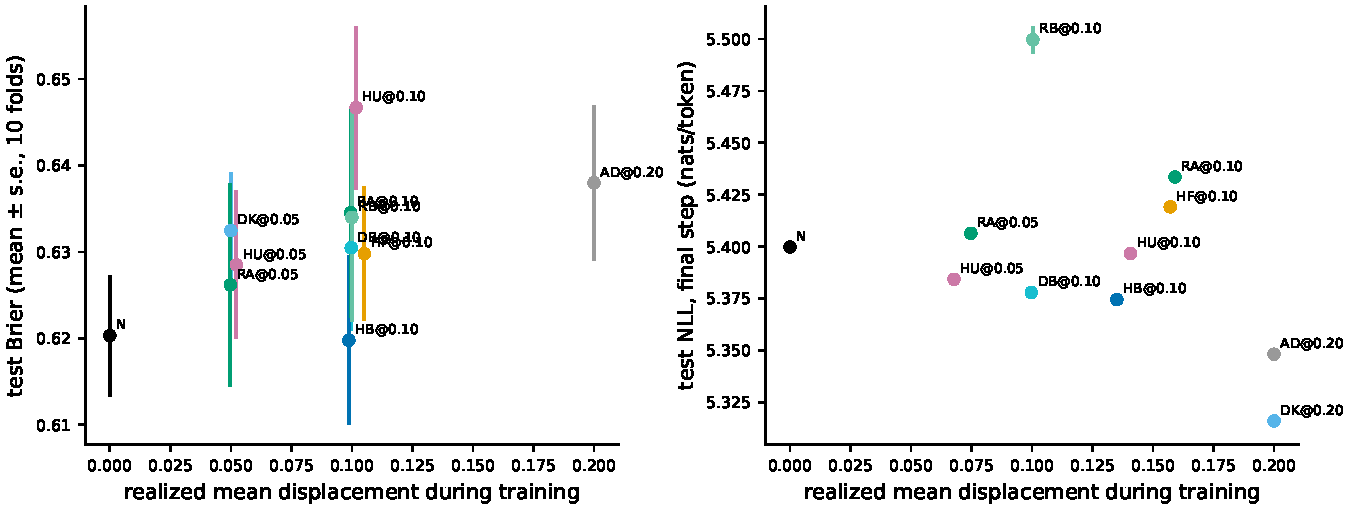
\includegraphics[width=\linewidth]{figures/fig_loss_vs_displacement.pdf}
\caption{Test loss against realized mean displacement recorded at the end of training. Left: encoder, test Brier
(mean $\pm$ s.e.\ over ten folds). Right: language model, final-step test NLL (mean over ten seeds). In the LM,
attention concentrates during training, so the realized displacement of the concentration-dependent arms (RA and
the top-4 deletion arms) at the last step exceeds the calibrated 0.10.}
\label{fig:dose}
\end{figure}

\paragraph{Encoder}
Attention regularization of any family changed little on PubMedQA. With no attention regularization, the
reference arm reached a test Brier of 0.620 and 67.0\% accuracy. Every calibrated attention arm lay between 0.620 and 0.647
Brier and between 64.9\% and 66.9\% accuracy. CapDrop matched the reference (0.620; 66.9\%), and no attention arm
improved on it. Every stabilized arm ran without failure or collapse (Figure~\ref{fig:strip}). Label smoothing and Mixout lowered
raw Brier through calibration (ECE 0.115 and 0.201, against about 0.30 for the attention arms). After temperature
scaling, all stabilized arms lay between 0.475 and 0.500. Discrimination was flat: macro AUROC ranged from 0.713 to 0.721.
The earlier LoRA recipe (L0) collapsed to the majority class in all ten folds. The question-only model (Q0) reached
49.3\% accuracy on its own question-only inputs, below the 55.2\% majority rate.

\begin{figure}[t]
\centering
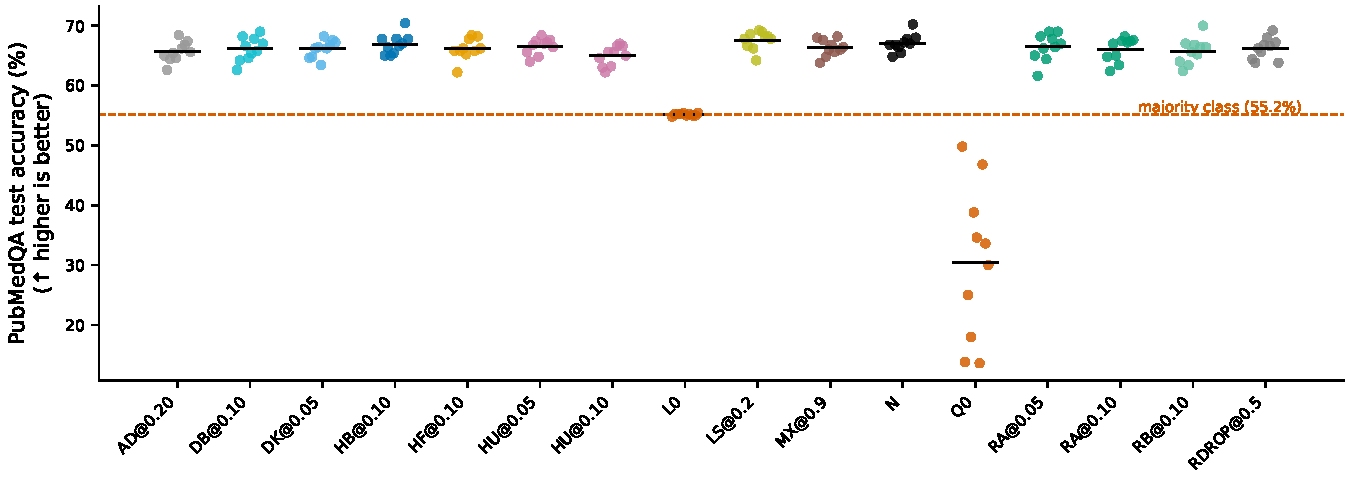
\includegraphics[width=\linewidth]{figures/fig_strip.pdf}
\caption{PubMedQA test accuracy of every run (ten folds per arm; bar: mean). Dashed: majority-class rate.
Q0 is shown on full inputs, a format it was not trained on; L0 collapses to the majority class.}
\label{fig:strip}
\end{figure}

\paragraph{Language model}
In the LM, CapDrop improved on the reference arm by 0.025 nats/token on every seed (descriptive; perplexity 215.8
versus 221.4). Fixed-$\alpha$ deletion and Relaxed Attention at $\ell=0.10$ made the reference worse, by 0.019 and
0.034. Part of the H1-L contrast is therefore harm done by HF, not only benefit from CapDrop. The two
best arms were attention dropout and DropKey at $\ell=0.20$ (5.348 and 5.316 nats/token; perplexity 203.6 for DropKey).
TV-budgeted relaxation was the worst (5.500). Validation curves (Figure~\ref{fig:lmcurves}) separate after about 500
steps and keep the same order to the end. By train-frequency bucket (descriptive), CapDrop's advantage over HF
comes from the four more frequent buckets (0.025--0.054 nats/token). On the rarest tokens it was 0.029 nats/token worse.

\begin{figure}[t]
\centering
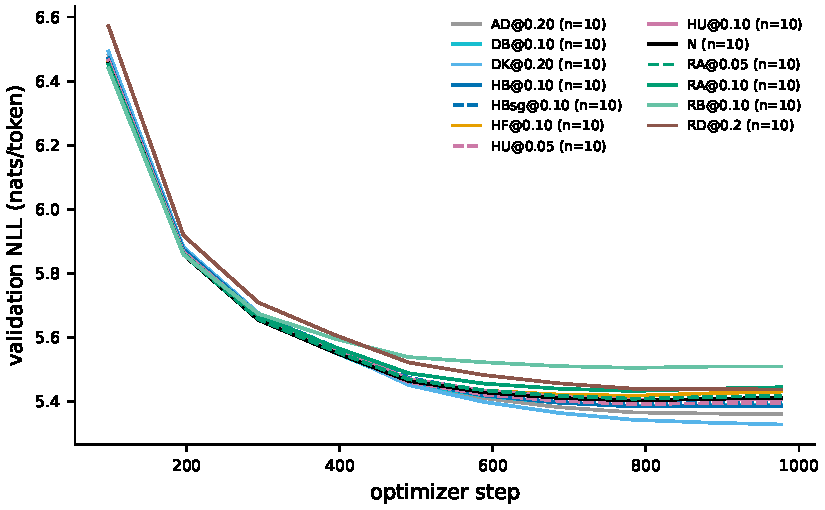
\includegraphics[width=0.8\linewidth]{figures/fig_lm_curves.pdf}
\caption{Language-model validation NLL during training, mean over ten seeds, for every arm run on all ten seeds.
Dashed: CapDrop with $\alpha$ under stop-gradient (E8) and the arms selected at $\ell=0.05$.}
\label{fig:lmcurves}
\end{figure}

\subsection{Evidence use on PubMedQA}\label{sec:evidence}
Figure~\ref{fig:evidence} shows that every fine-tuned model uses the abstract, mostly through its RESULTS section,
and that attention regularization does not change how. The evidence-use gap (full minus question-only accuracy) was
11.6--16.0 points for the stabilized arms. Their question-only accuracy (51--53\%) fell below the majority rate.
Deleting the RESULTS section lowered accuracy to 55--56\%, the majority rate. A label-differing abstract from
another question flipped 55--63\% of predictions, and about 57\% of predictions then followed the donor abstract's label.
CapDrop did not differ from the reference in evidence-use gap ($-1.2$ points) or flip rate ($+1.1$ points).

\begin{figure}[t]
\centering
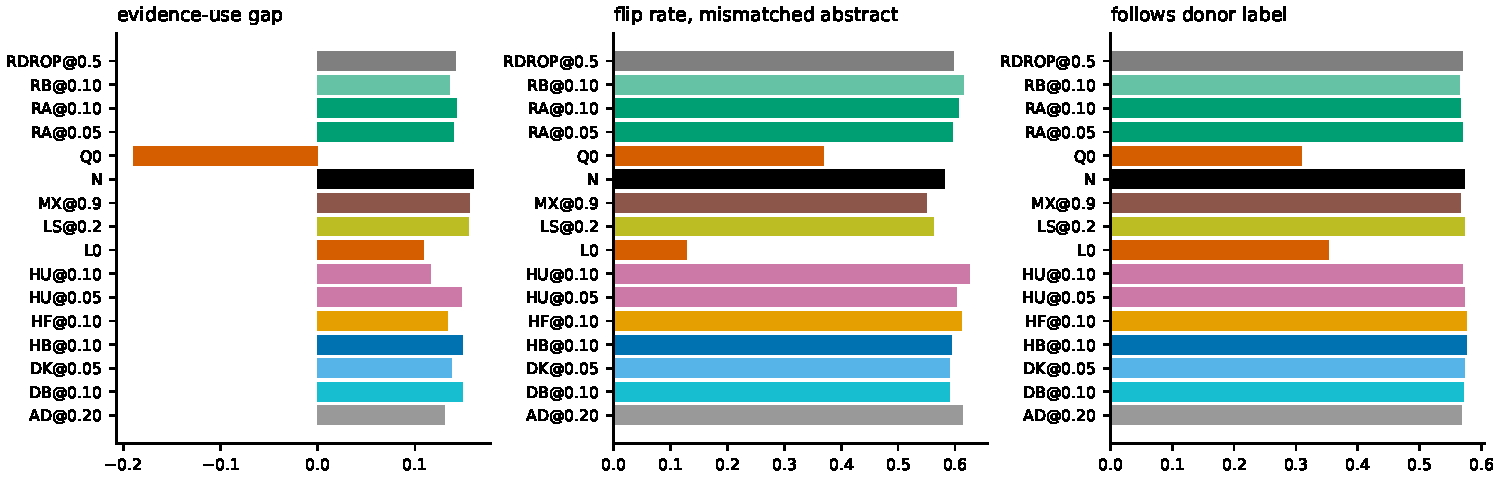
\includegraphics[width=\linewidth]{figures/fig_evidence.pdf}
\caption{PubMedQA evidence-use diagnostics on the test set (mean over ten folds). Left: evidence-use gap. Middle:
fraction of predictions that change when the abstract is replaced by one with a different gold label. Right: fraction
of predictions equal to the donor abstract's label.}
\label{fig:evidence}
\end{figure}

\subsection{Extensions}\label{sec:extresults}
Every declared extension except E6 ran to completion within the cap. Table~\ref{tab:extensions} gives the contrasts.

% Generated by tables_results.py from results/analysis.json; do not edit by hand.
\begin{table}[t]
\centering
\caption{Extension contrasts (descriptive; unadjusted $p$, verdicts by the H1 rules). Encoder rows: test Brier (E4:
SciFact development set used once as a test), 95\% two-level bootstrap CI, co-criterion = TS-Brier difference.
LM rows: final-step test NLL; $^\dagger$90\% paired-$t$ interval used for equivalence (margin $\pm0.010$);
co-criterion = best-validation-step difference. Differences are first arm minus second arm; lower is better, so a
negative difference favours the first arm. E2 (failure rates) is reported in the text; E6 was not run (budget).}
\label{tab:extensions}
\footnotesize
\setlength{\tabcolsep}{3pt}
\resizebox{\linewidth}{!}{\begin{tabular}{lllcccl}
\toprule
Extension & Contrast & Diff. & CI & Co-crit. & $p$ & Verdict\\
\midrule
P1 (seed 2) & HB@0.10 $-$ HF@0.10 & $-$0.001 & [$-$0.024, +0.021] & +0.000 & 0.916 & Inconclusive\\
B6 OOF, H2-E & HB@0.10 $-$ RA@0.05 & +0.004 & [$-$0.017, +0.025] & +0.001 & 0.562 & Inconclusive\\
B6 OOF, H3-E & HB@0.10 $-$ LS@0.2 & +0.131 & [+0.103, +0.160] & +0.008 & 0.008 & calibration only\\
E-S3 & S-HB@0.10 $-$ S-HF@0.10 & +0.010 & [$-$0.004, +0.026] & +0.007 & 0.061 & Inconclusive\\
E-S3 & S-N $-$ S-noKD & +0.014 & [$-$0.038, +0.065] & +0.010 & 0.031 & Inconclusive\\
E5 BioLinkBERT & HB@0.10 $-$ HU@0.10 & +0.001 & [$-$0.021, +0.023] & $-$0.000 & 0.930 & Inconclusive\\
E5 BioLinkBERT & HB@0.10 $-$ N & +0.006 & [$-$0.013, +0.027] & +0.005 & 0.305 & Inconclusive\\
E5 BioLinkBERT & HU@0.10 $-$ N & +0.006 & [$-$0.017, +0.030] & +0.005 & 0.492 & Inconclusive\\
E5 BioLinkBERT & AD@0.20 $-$ N & $-$0.001 & [$-$0.026, +0.025] & +0.000 & 0.951 & Inconclusive\\
E4 SciFact & HB@0.10 $-$ HU@0.10 & +0.028 & [+0.005, +0.051] & +0.007 & 0.020 & calibration only\\
E4 SciFact & HB@0.10 $-$ N & +0.022 & [$-$0.005, +0.052] & +0.026 & 0.045 & Inconclusive\\
E4 SciFact & HU@0.10 $-$ N & $-$0.007 & [$-$0.040, +0.028] & +0.019 & 0.609 & Inconclusive\\
E4 SciFact & RA@0.05 $-$ N & +0.019 & [+0.001, +0.037] & +0.018 & 0.004 & Worse\\
E1 R-Drop & HB@0.10 $-$ RDROP@0.5 & $-$0.013 & [$-$0.040, +0.014] & $-$0.009 & 0.287 & Inconclusive\\
E3 (encoder) & DB@0.10 $-$ HB@0.10 & +0.011 & [$-$0.012, +0.035] & +0.006 & 0.295 & Inconclusive\\
E3 (LM) & DB@0.10 $-$ HB@0.10 & +0.003 & [+0.002, +0.005]$^\dagger$ & +0.002 & 0.012 & Equivalent\\
E8 (LM) & HBsg@0.10 $-$ HB@0.10 & +0.010 & [+0.008, +0.011]$^\dagger$ & +0.010 & 0.002 & Worse\\
\bottomrule
\end{tabular}}
\end{table}


\paragraph{Second seed, out-of-fold replication and second encoder}
The second seed (P1) gave the same H1-E picture, with a difference of $-0.001$ Brier. The out-of-fold replication of the
encoder selection on folds 2--9 reproduced the H2-E and H3-E verdicts. With BioLinkBERT (E5), no contrast differed from zero,
and HB$-$HU was $+0.001$.

\paragraph{Second task (E4, SciFact)}
On SciFact, CapDrop's raw Brier was higher than unbudgeted deletion's by 0.028. The difference vanished after temperature
scaling ($+0.007$), so this too is calibration only, with the opposite sign to the PubMedQA encoder.
Relaxed Attention was worse than the reference by 0.019 Brier on both criteria. Under the replication rule, neither E4 nor E5
reproduces the H1-E verdict.

\paragraph{Fragile recipe (E2)}
Under the original BERT recipe, attention dropout failed (test accuracy at most the majority rate) in 19 of 20 runs.
CapDrop and Mixout each failed in 15 of 20. The reduction of 20 points was not significant for either arm
(Holm $p=0.22$; 90\% intervals $[0, 40]$ and $[5, 40]$ points). The upper bounds exceed 25 points, so ``no reduction''
cannot be claimed either. The comparison is inconclusive.

\paragraph{Distilled students (E-S3)}
The privileged teachers passed their gate (70.8\% pooled out-of-fold accuracy on folds 0--4). The reference
student passed its gate too (58.8\%), so S-a and S-b entered the secondary family (above). Students kept 91.2--92.8\% of the
full model's PubMedQA accuracy with 61\% of its parameters. At 384 tokens they halve batch-1 latency on the GPU
(5.9 versus 11.1\,ms) and on four CPU threads (112 versus 226\,ms), and double GPU throughput (326 versus 166 sequences/s).
Distillation itself did not measurably change Brier (S-N$-$S-noKD: $+0.014$, interval $[-0.038, 0.065]$).

\paragraph{R-Drop (E1) and targeting (E3)}
R-Drop with the selected $\alpha=0.5$ did not differ from CapDrop ($-0.013$ Brier, $p=0.29$) and took 2.4 times
as long to train. Budgeted DropKey, which applies the same cap to a candidate that may delete any key, was
indistinguishable from CapDrop in the encoder. In the LM it was equivalent within $\pm0.010$ nats/token
($+0.003$; 90\% interval $[0.002, 0.005]$).

\paragraph{Gradient path (E8)}
CapDrop's gradient flows through $\alpha=\min(1,\tau/m)$, and fixed-$\alpha$ deletion has no such path. E8 removes the path
by computing $\alpha$ under stop-gradient, which leaves the forward pass and every deletion draw unchanged. This raised test NLL by
0.0097 nats/token on every seed (90\% interval $[0.008, 0.011]$; best-validation step 0.010; descriptive). The
detached variant still beat fixed-$\alpha$ deletion by 0.035 and unbudgeted deletion by 0.013 nats/token, again on every
seed (descriptive, paired by seed). About four fifths of the H1-L difference therefore comes with the capped forward
perturbation itself, and about one fifth with the gradient through $\alpha$.

\paragraph{E6}
The single-epoch LM extension (E6) was not run. After E3, 85.1 GPU-hours had been used, and E6's expected 5.6 GPU-hours
would have exceeded the 90-hour cap. E8 (1.25 GPU-hours) fitted under the cap and was run.

\subsection{Audits, exploratory analyses and compute}\label{sec:audits}
Two runs per regime, chosen by a hash of the protocol, were retrained twice in deterministic mode. Each pair agreed exactly
(maximum difference 0) and produced identical sealed files. The original non-deterministic runs agreed with the
replays within the registered tolerance (largest deviation 0.010 dev Brier against a tolerance of 0.137). Evaluation
replays from saved checkpoints were bit-identical.

Exploratory analyses were as follows. The encoder dose--response over matched pairs was flat (Spearman $\rho=-0.24$, $p=0.71$, six
points). Brown--Forsythe tests found no difference in between-fold variance between CapDrop and HF, HU, RA or N ($p\ge0.28$). The descriptive
displacement-accounting model (per-run test Brier on realized $\bar D$, realized $S_2$, census $B$ and fold effects,
fitted on N, AD, DK and RA) had $R^2=0.85$ including fold effects. It predicted the HU, HF, HB and RB arms within
0.012 Brier. It is not a mediation analysis.

The campaign used 86.3 GPU-hours of compute (thermal pauses excluded) on one 4\,GB laptop GPU, within the 90-hour
cap. Every declared run completed and none was cut. The only replaced runs are the three DropKey LM tuning runs
that were excluded before any test outcome was seen (Section~
ef{sec:discussion}).
